\subsection{Testing Plans}

\subsubsection{Variations from initial plans}
Originally, it was planned to use pressure sensors to determine the amount of force that is applied when the skater uses their feet to push off of the ground and how their weight is being distributed during various actions. It was determined that the pressure sensors do not accurately detect the desired results, resulting in load sensors to be used instead. The load sensors accurately determine the same result that was wanted from the pressure sensors. Eight load sensors will be used in total, with four load sensors that will be used for each foot.

A total of six EMG sensors were determined to be used to execute the testing of the muscle activity. Three EMG sensors will be placed on each leg of the test subject, with a common reference node on the ankle. The specific placements of the EMG sensors were determined through research and experimentation. The EMG sensors will be placed on the Vastus Lateralis (quadriceps muscle), Gastrocnemius (flexor muscle), and the Bicep Femoris (hamstring muscle), highlighted below in figure 4.1\cite{1}. The Vastus Lateralis  muscle is located on the outside of the quadriceps muscle group. The Vastus Lateralis is greatly used while playing hockey, as it is the muscle that applies the force on the ice that is used to push the skater forward\cite{2}. The Gastrocnemius muscle is one of the main muscles within the calf and is a part of the flexor muscle group. The Gastrocnemius muscle is important, like the Vastus Lateralis in propelling the skater forward. As well, it is important in acceleration of the skater as it extends the foot when the stride is complete \cite{2}. The Bicep Femoris muscle is located on the posterior compartment of the thigh and is one of the muscles within the hamstring muscle group. The Bicep Femoris muscle is the main muscle that points the foot outward, which makes it important in the positioning of the skater's feet when skating\cite{2}. 
\par
\begin{figure}[htb]
\centering
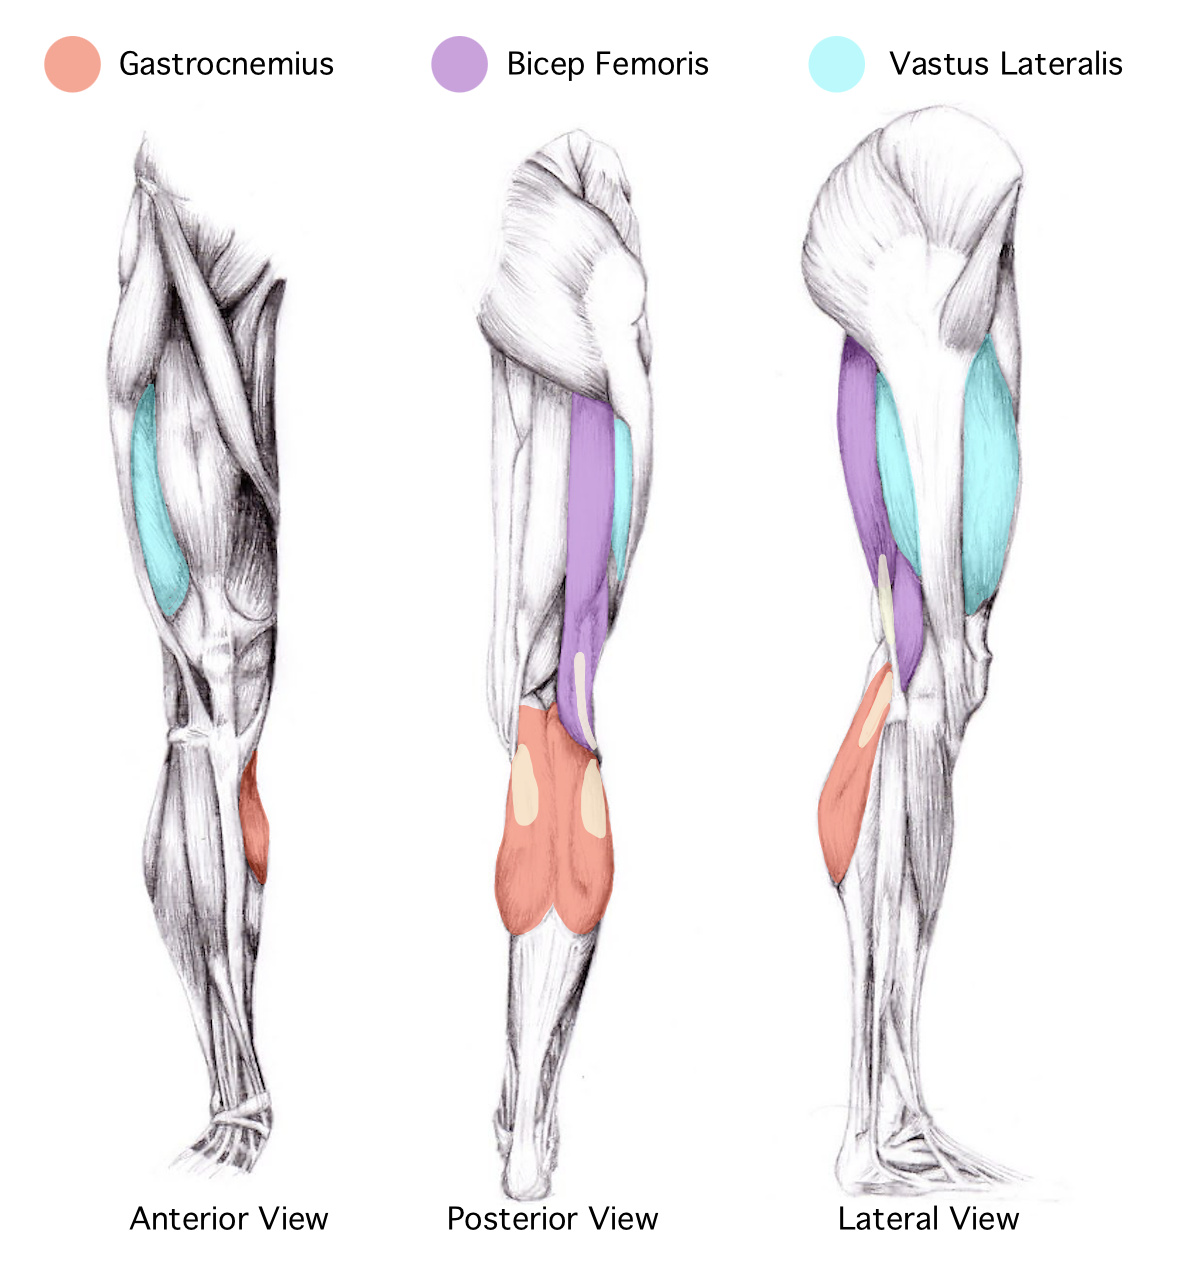
\includegraphics[scale=0.5]{Progress_Report/figs/highlightedmuscles.png}
\caption{Diagram of the Leg Muscles that will be Tested (highlighted are the muscles that will be tested)\cite{3}}
\label{fig:Muscles}
\end{figure}
\par


The Vastus Lateralis muscle is expected to have the greatest activity when the test subject is skating at a steady-state. The Gastrocnemius muscle is expected to have the greatest activity when the test subject is skating in order to increase their acceleration. The Bicep Femoris is expected to have the greatest activity when the test subject is skating at a steady-state.

\subsubsection{Progress}
For the testing we have a very limited amount of time of only 50 minutes on the ice so we need to be a quick and concise as possible as we will be going over multiple drills in order to capture the correct data of the skater. These drills will be both the same for indoor roller skating and our on-ice hockey. For the testing we will have five drills with varying intensity and muscles being targeting for our EMG sensors. These five drills will be our cross-over drill, stopping drill, laps around, forwards and backwards drill, and shooting. These drill can be observed in Figure 4.2.
\par
\begin{figure}[H]
\centering
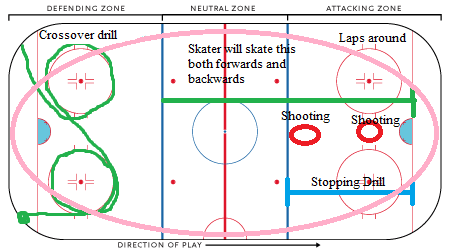
\includegraphics{Progress_Report/figs/HockeyRink-Zones.png}
\caption{Breakdown of the five drill participants will be demonstrating\cite{4}}
\label{fig:HockeyRink}
\end{figure}
\par
The cross-over drill is a high-intensity drill that involves the participant going around the circles located at the ends of the ice rink. This drill with have the participant go around the circle once then at continue on to the next circle going around it once. This drill will give the team a good indication of the force being exerted during, and the angle at which the skater is at relative to the ice. The next drill will then have the participant conducting the cross-over drill backwards. 

For the stopping drill, the participant will start at the goal line from rest and then accelerate to the blue line, where they will then stop. This drill is focused on the participant's force used in order to stop. 

The third drill will require the participant to skate laps around the rink. This is a lower intensity drill meant to focus on the EMG sensors that are placed on the test subject's legs, rather than the load sensors. The EMG sensors will be placed on the Vastus Lateralis, Gastrocnemius, and Bicep Femoris muscles. The low intensity drill will ensure that the activity of these three muscles can be accurately observed in steady-state skating, as well as accelerated skating. 

For the fourth drill this will be the forwards and backwards drill, the participant will start at the goal line and then skate forwards to the far blue line before stopping and then skating backwards, this will show the participants muscles and pressure sensors when they stop and start back up when the participant starts skating backwards. This drill will give us a good reading on the muscles used to stop and start and going from forwards to backwards. 

The final drill will be our shooting drill, this drill will be from two different locations, on from the hash-marks, the other from the blue line, each participant will get ten hockey pucks to shoot with. For these drills the placement of the EMG sensors will be changed to the lower back and arm muscles, the pressure sensors will stay in the same location and the angle with the gyroscope that the participant shoots at will be observed. The back and arm muscles that the EMG sensors will be placed on are the Latissimus Dorsi, Anterior Deltoid, and the Brachioradialis, displayed below in figure 4.3\cite{5}. The reference node for the EMG sensors on the back and arm will be placed on a spinous process.  
\par
\begin{figure}[htb]
\centering
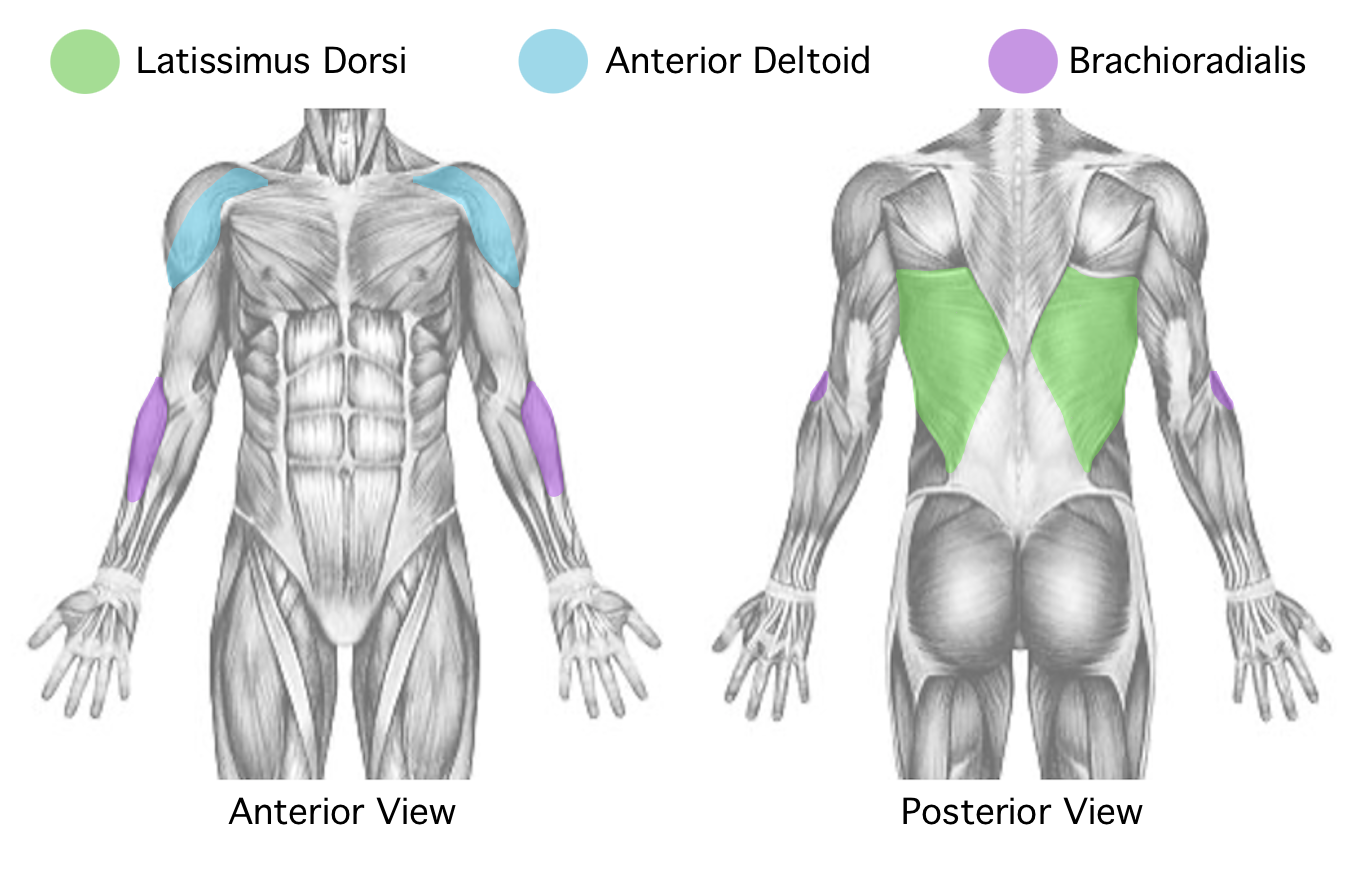
\includegraphics[scale=0.5]{Progress_Report/figs/shootingmuscles.png}
\caption{Diagram of the Back and Arm Muscles that will be Tested (highlighted are the muscles that will be tested)\cite{6}}
\label{fig:ShootingMuscles}
\end{figure}
\par
The Latissimus Dorsi muscle is a core muscle that is found on the lower back. The Latissimus Dorsi is an important muscle that contributed to the abduction, extension, and rotation of the arm\cite{5}. The Anterior Deltoid is a muscle that is found within the shoulder and contributes to the flexion of the arm and the rotation of the shoulder\cite{5}. The Anterior Deltoid is majorly used while in hockey for shooting and passing the puck\cite{7}. The Brachioradialis muscle is found in the forearm and is important in the bending and flexing of the elbow\cite{5}. The Brachioradialis is used in hockey for shooting the puck, as well as for control of the hockey stick\cite{7}.
